\documentclass[a4paper,11pt]{article}
\input{/home/tof/Documents/Cozy/latex-include/preambule_lua.tex}
\newcommand{\showprof}{show them}  % comment this line if you don't want to see todo environment
\fancyhead[L]{Tri par tas}
\newdate{madate}{10}{09}{2020}
%\fancyhead[R]{\displaydate{madate}} %\today
%\fancyhead[R]{Seconde - SNT}
%\fancyhead[R]{Première - NSI}
\fancyhead[R]{Terminale - NSI}
\fancyfoot[L]{~\\Christophe Viroulaud}
\AtEndDocument{\label{lastpage}}
\fancyfoot[C]{\textbf{Page \thepage/\pageref{lastpage}}}
\fancyfoot[R]{\includegraphics[width=2cm,align=t]{/home/tof/Documents/Cozy/latex-include/cc.png}}
\usepackage{tikz}

\begin{document}
\begin{Form}
\section{Problématique}
Trier efficacement est une tâche fondamentale en algorithmique.
\begin{center}
\shadowbox{\parbox{16cm}{\centering Peut-on trier un tableau efficacement en utilisant les propriétés des arbres binaires?}}
\end{center}
\section{Un tas}
\subsection{Définition}
Un \textbf{arbre partiellement ordonné} est tel que la valeur de chaque nœud fils est inférieur au nœud père (figure \ref{apo}).
\begin{center}
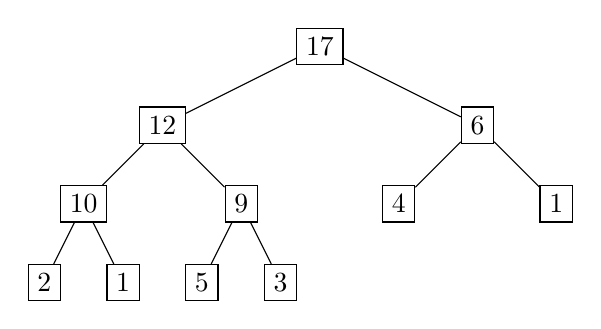
\begin{tikzpicture}
\node[draw] (0) at (0,0) {17};
\node[draw] (1) at (-2,-1) {12};
\node[draw] (2) at (2,-1) {6};
\node[draw] (3) at (-3,-2) {10};
\node[draw] (4) at (-1,-2) {9};
\node[draw] (5) at (1,-2) {4};
\node[draw] (6) at (3,-2) {1};
\node[draw] (7) at (-3.5,-3) {2};
\node[draw] (8) at (-2.5,-3) {1};
\node[draw] (9) at (-1.5,-3) {5};
\node[draw] (10) at (-0.5,-3) {3};
\draw (0) -- (1);
\draw (0) -- (2);
\draw (1) -- (3);
\draw (1) -- (4);
\draw (2) -- (5);
\draw (2) -- (6);
\draw (3) -- (7);
\draw (3) -- (8);
\draw (4) -- (9);
\draw (4) -- (10);
\end{tikzpicture}
\captionof{figure}{Arbre partiellement ordonné}
\label{apo}
\end{center}
\begin{commentprof}
Un arbre partiellement ordonné n'implique pas que tous les éléments soient ordonnés.
\end{commentprof}
Un \textbf{tas} est un tableau dont l'arbre associé est un arbre partiellement ordonné (code \ref{tas}).
\begin{center}
\begin{lstlisting}[language=Python]
tas = [17, 12, 6, 10, 9, 4, 1, 2, 1, 5, 3]
\end{lstlisting}
\captionof{code}{Tas associé à l'arbre \ref{apo}}
\label{tas}
\end{center}
Chaque nœud fils est accessible en respectant la convention suivante:
\begin{itemize}
\item l'indice de la racine est 0,
\item l’indice du fils gauche est 2 ∗ i + 1,
\item l’indice du fils droit est 2 ∗ i + 2.
\end{itemize}
\begin{activite}
Écrire la fonction \textbf{echanger(t: list, i1: int, i2: int)$\;\rightarrow\;$None} qui inverse les éléments d'indice \emph{i1} et \emph{i2} du tableau \emph{t}.
\end{activite}
\subsection{Tamiser un élément du tableau}
Un tableau n'est pas nécessairement un tas (figure \ref{tamis0}).
\begin{center}
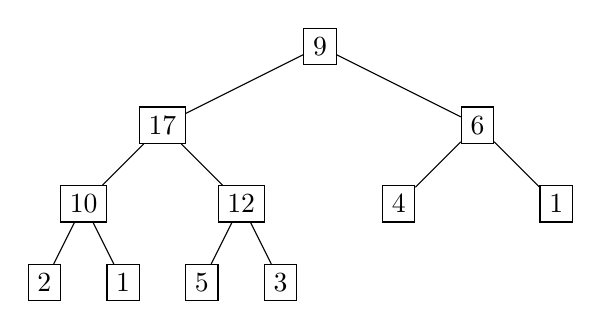
\begin{tikzpicture}
\node[draw] (0) at (0,0) {9};
\node[draw] (1) at (-2,-1) {17};
\node[draw] (2) at (2,-1) {6};
\node[draw] (3) at (-3,-2) {10};
\node[draw] (4) at (-1,-2) {12};
\node[draw] (5) at (1,-2) {4};
\node[draw] (6) at (3,-2) {1};
\node[draw] (7) at (-3.5,-3) {2};
\node[draw] (8) at (-2.5,-3) {1};
\node[draw] (9) at (-1.5,-3) {5};
\node[draw] (10) at (-0.5,-3) {3};
\draw (0) -- (1);
\draw (0) -- (2);
\draw (1) -- (3);
\draw (1) -- (4);
\draw (2) -- (5);
\draw (2) -- (6);
\draw (3) -- (7);
\draw (3) -- (8);
\draw (4) -- (9);
\draw (4) -- (10);
\end{tikzpicture}
\captionof{figure}{La racine ne respecte pas les propriétés du tas}
\label{tamis0}
\end{center}
Tamiser un élément du tableau consiste à faire respecter la propriété d'un arbre partiellement ordonné pour ce nœud. Prenons l'exemple du nœud racine contenant la valeur 9. Pour respecter la propriété il faut échanger la valeur du nœud père (9) avec la valeur de son plus grand fils (17).
\begin{center}
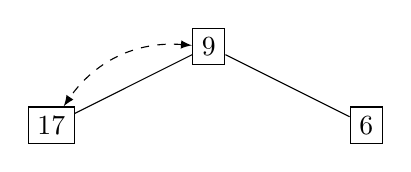
\begin{tikzpicture}
\node[draw] (0) at (0,0) {9};
\node[draw] (1) at (-2,-1) {17};
\node[draw] (2) at (2,-1) {6};
\draw (0) -- (1);
\draw (0) -- (2);
\draw[<->,>=latex,dashed] (0) to[bend right] (1);
\end{tikzpicture}
\captionof{figure}{Échange du père avec son plus grand fils.}
\label{tamis1}
\end{center}
\begin{center}
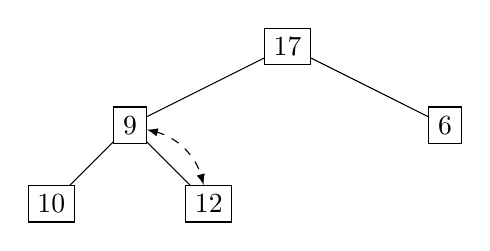
\begin{tikzpicture}
\node[draw] (0) at (0,0) {17};
\node[draw] (1) at (-2,-1) {9};
\node[draw] (2) at (2,-1) {6};
\node[draw] (3) at (-3,-2) {10};
\node[draw] (4) at (-1,-2) {12};
\draw (0) -- (1);
\draw (0) -- (2);
\draw (1) -- (3);
\draw (1) -- (4);
\draw[<->,>=latex,dashed] (1) to[bend left] (4);
\end{tikzpicture}
\captionof{figure}{Propagation récursive}
\label{tamis2}
\end{center}
\begin{center}
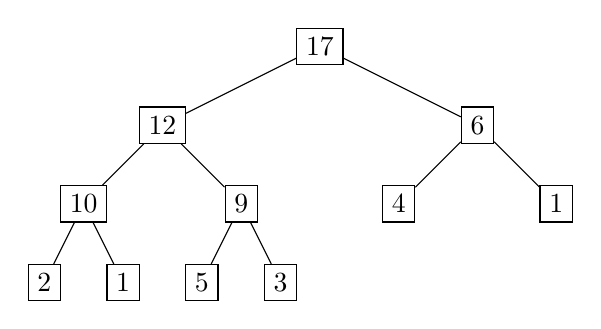
\begin{tikzpicture}
\node[draw] (0) at (0,0) {17};
\node[draw] (1) at (-2,-1) {12};
\node[draw] (2) at (2,-1) {6};
\node[draw] (3) at (-3,-2) {10};
\node[draw] (4) at (-1,-2) {9};
\node[draw] (5) at (1,-2) {4};
\node[draw] (6) at (3,-2) {1};
\node[draw] (7) at (-3.5,-3) {2};
\node[draw] (8) at (-2.5,-3) {1};
\node[draw] (9) at (-1.5,-3) {5};
\node[draw] (10) at (-0.5,-3) {3};
\draw (0) -- (1);
\draw (0) -- (2);
\draw (1) -- (3);
\draw (1) -- (4);
\draw (2) -- (5);
\draw (2) -- (6);
\draw (3) -- (7);
\draw (3) -- (8);
\draw (4) -- (9);
\draw (4) -- (10);
\end{tikzpicture}
\captionof{figure}{La valeur 9 est à sa place}
\label{tamis3}
\end{center}
\begin{activite}
\begin{enumerate}
\item Écrire la fonction \emph{récursive} \textbf{tamiser(t: list, i\_pere: int)$\;\rightarrow\;$None} qui positionne correctement le nœud d'indice \emph{i\_pere}.
\item Tester avec le tableau associé à la figure \ref{tamis0}.
\item Modifier la signature de la fonction tel que \textbf{tamiser(t: list, i\_pere: int, i\_max: int)$\;\rightarrow\;$None} afin qu'elle ne tamise que jusqu'à l'indice \emph{i\_max} (inclus) et non plus jusqu'à la fin du tableau. Cette propriété nous sera utile lors du tri.
\end{enumerate}
\end{activite}
\subsection{Entasser le tableau}
En tamisant chaque élément du tableau, on obtient un tas. Une bonne approche est de commencer par le bas de l'arbre. Ainsi, les sous-arbres droit et gauche respectent toujours la propriété d'un arbre partiellement ordonné. De plus, une feuille respectant nécessairement la propriété, il est judicieux de ne commencer qu'au premier nœud qui n'est pas une feuille.
\begin{activite}
Écrire la fonction \textbf{entasser(t: list)$\;\rightarrow\;$None} qui transforme le tableau \emph{t} en tas, en tamisant chaque nœud (qui n'est pas une feuille).
\end{activite} 
\section{Principe du tri par tas}
Dans un tas la racine contient la plus grande valeur. Il suffit alors d'inverser cette valeur avec la dernière du tableau pour la placer définitivement. Il suffit ensuite d'appliquer le même principe au reste du tableau.
\begin{center}
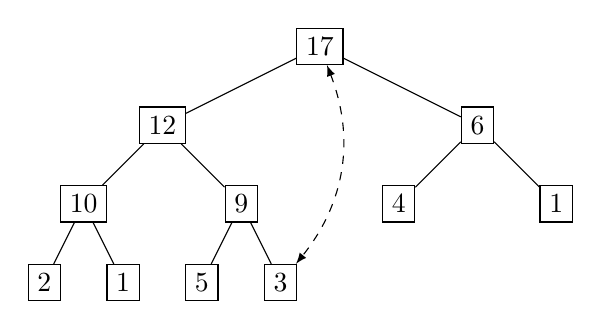
\begin{tikzpicture}
\node[draw] (0) at (0,0) {17};
\node[draw] (1) at (-2,-1) {12};
\node[draw] (2) at (2,-1) {6};
\node[draw] (3) at (-3,-2) {10};
\node[draw] (4) at (-1,-2) {9};
\node[draw] (5) at (1,-2) {4};
\node[draw] (6) at (3,-2) {1};
\node[draw] (7) at (-3.5,-3) {2};
\node[draw] (8) at (-2.5,-3) {1};
\node[draw] (9) at (-1.5,-3) {5};
\node[draw] (10) at (-0.5,-3) {3};
\draw (0) -- (1);
\draw (0) -- (2);
\draw (1) -- (3);
\draw (1) -- (4);
\draw (2) -- (5);
\draw (2) -- (6);
\draw (3) -- (7);
\draw (3) -- (8);
\draw (4) -- (9);
\draw (4) -- (10);
\draw[<->,>=latex,dashed] (0) to[bend left] (10);

\end{tikzpicture}
\captionof{figure}{Placer le plus grand élément en fin.}
\label{apo}
\end{center}
\begin{center}
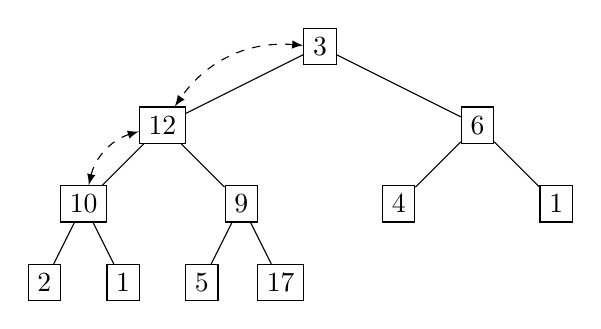
\begin{tikzpicture}
\node[draw] (0) at (0,0) {3};
\node[draw] (1) at (-2,-1) {12};
\node[draw] (2) at (2,-1) {6};
\node[draw] (3) at (-3,-2) {10};
\node[draw] (4) at (-1,-2) {9};
\node[draw] (5) at (1,-2) {4};
\node[draw] (6) at (3,-2) {1};
\node[draw] (7) at (-3.5,-3) {2};
\node[draw] (8) at (-2.5,-3) {1};
\node[draw] (9) at (-1.5,-3) {5};
\node[draw] (10) at (-0.5,-3) {17};
\draw (0) -- (1);
\draw (0) -- (2);
\draw (1) -- (3);
\draw (1) -- (4);
\draw (2) -- (5);
\draw (2) -- (6);
\draw (3) -- (7);
\draw (3) -- (8);
\draw (4) -- (9);
\draw (4) -- (10);
\draw[<->,>=latex,dashed] (0) to[bend right] (1);
\draw[<->,>=latex,dashed] (1) to[bend right] (3);
\end{tikzpicture}
\captionof{figure}{Tamiser.}
\label{apo}
\end{center}
\begin{center}
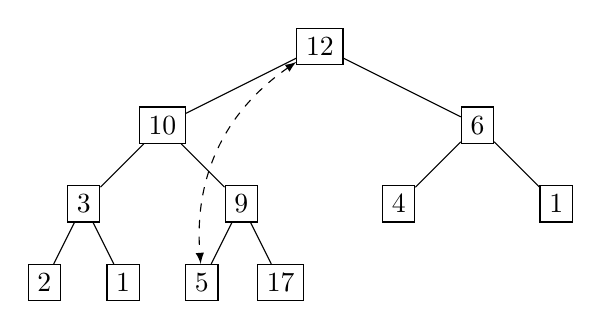
\begin{tikzpicture}
\node[draw] (0) at (0,0) {12};
\node[draw] (1) at (-2,-1) {10};
\node[draw] (2) at (2,-1) {6};
\node[draw] (3) at (-3,-2) {3};
\node[draw] (4) at (-1,-2) {9};
\node[draw] (5) at (1,-2) {4};
\node[draw] (6) at (3,-2) {1};
\node[draw] (7) at (-3.5,-3) {2};
\node[draw] (8) at (-2.5,-3) {1};
\node[draw] (9) at (-1.5,-3) {5};
\node[draw] (10) at (-0.5,-3) {17};
\draw (0) -- (1);
\draw (0) -- (2);
\draw (1) -- (3);
\draw (1) -- (4);
\draw (2) -- (5);
\draw (2) -- (6);
\draw (3) -- (7);
\draw (3) -- (8);
\draw (4) -- (9);
\draw (4) -- (10);
\draw[<->,>=latex,dashed] (0) to[bend right] (9);
\end{tikzpicture}
\captionof{figure}{Recommencer.}
\label{apo}
\end{center}
\begin{activite}
Écrire la fonction \textbf{tri\_par\_tas(t: list)$\;\rightarrow\;$None} qui implémente l'algorithme ci-après:
\begin{itemize}
\item Entasser le tableau.
\item Initialiser indice\_dernier.
\item Tant que indice\_dernier \geq 0
\begin{itemize}
\item Échanger le premier élément avec l'élément d'indice indice\_dernier.
\item Tamiser le tableau de la racine jusqu'à l'élément d'indice indice\_dernier.
\item Décrémenter indice\_dernier.
\end{itemize}
\end{itemize}
\end{activite}
Ce tri a une complexité temporelle en $O(n.log(n))$
\end{Form}
\end{document}